\newpage
\begin{center}
  \textbf{\large 2. РАЗРАБОТКА И РЕАЛИЗАЦИЯ АЛГОРИТМА}
\end{center}
\refstepcounter{chapter}
\addcontentsline{toc}{chapter}{2. РАЗРАБОТКА И РЕАЛИЗАЦИЯ АЛГОРИТМА}


\section{Описание проблемы}

Доказано в  работе \cite{zakharova2022integer}, что проблема формирования групп обучающихся на курсах дополнительного образования является NP - сложной даже в том случае, когда необходимо составить оптимальное расписание только по одной дисциплине при условии, что каждый преподаватель может надежно работать в любой доступный промежуток времени.Также в работе \cite{zakharova2022integer} приведено доказательство теоремы о том, что проблема формирования групп учащихся на курсах дополнительного образования является NP - сложной даже в том случае, когда и преподаватели, и учащиеся доступны для индивидуальных занятий во все временные интервалы, но ненадежность преподавателей играет определенную роль.


Этапы работы над реализацией алгоритма “жадного” типа
\begin{enumerate}
    \item Проектирование алгоритма
    \item Написание алгоритма на языке Python
    \item Тестирование алгоритма на тестовых данных
    \item Отладка и улучшение алгоритма “жадного” типа
    \item Тестирование алгоритма на данных профориентационной школы
    \item Отладка и улучшение алгоритма
\end{enumerate}



\section{Описание предлагаемого алгоритма для распределения учащихся и составления групп}

Для составления расписания и распределения по группам, используется следующий алгоритм, описанный в []

У нас есть следующие входные наборы:

D = {d} – набор дисциплин;

Ξ = {θ} – множество временных интервалов;

C = {c} — множество классов;

M = {m} — набор обучающихся;

K = {k} — множество учителей.

Дисциплины Dk и подмножество временных интервалов Ξk, допустимых для работы. Пусть Cτ обозначает подмножество классных комнат, доступных во временном интервале τ, а Cd — подмножество классных комнат, подходящих для дисциплины d. Для обучающегося m задано подмножество обязательных дисциплин Dm и подмножество предпочтительных временных интервалов Ξm.
Необходимо сформировать образовательные группы путем распределения дисциплин, учителей и учащихся по временным интервалам и классам при следующих ограничениях. Количество групп, назначенных учителю k, должно находиться в диапазоне от n(k) до N(k). Размер группы, находящейся в классе c, имеет нижнюю границу min(c) и верхнюю границу max(c). Разнообразие дисциплины d (количество активных временных интервалов) должно быть не менее заданного параметра V(d). Уровень ненадежности w(k,τ) указан для каждой пары учителей и временного интервала из-за других действий учителя. Для стабильной работы курсов суммарная ненадежность должна быть меньше порога U(τ) в интервале времени τ. Цель состоит в том, чтобы максимизировать взвешенную сумму учащихся, распределенных по группам. Здесь мы вводим вес a(m, d), чтобы указать важность учащегося m и его предпочтение дисциплине d.

Основная идея модели заключается в составлении таких объектов, как обучающийся по каждой требуемой дисциплине и преподаватель по каждой предпочтительной дисциплине. Эти объекты распределяются по временным интервалам с использованием имеющихся аудиторий \begin{figure}[!ht]
  \centering
  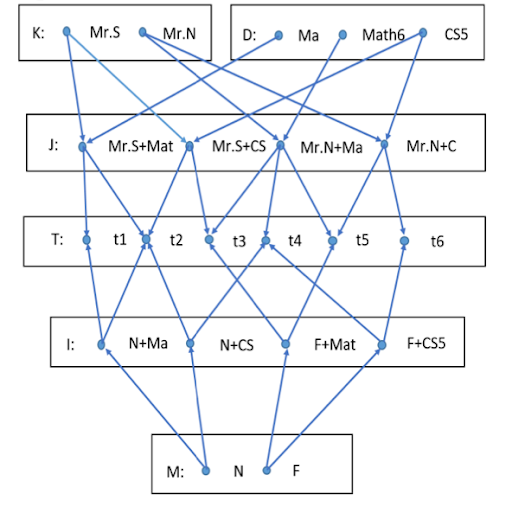
\includegraphics[width=100mm]{Images/alg_1.png}
  \caption{\textbf{}}
  \label{alg1}
\end{figure} (см. пример на \ref{alg1}).


Введем следующие обозначения:
\begin{itemize}
    \item Т = {t1, . . . , tl} — набор классных часов для работы с обучающимися;
    \item G(τ) — подмножество классных часов, соответствующих к временному интервалу τ;
    \item I = {i} – множество пар: обучающийся и дисциплина;
    \item P(m) – набор пар i (учащийся и дисциплина), соответствующих ответ учащемуся m;
    \item T (i) — подмножество временных интервалов в классе, доступных для i;
    \item a(i) — весовой коэффициент для учащегося с дисциплиной - пара i;
    \item J = {j} – множество пар: преподаватель и дисциплина;
    \item M(k) – множество пар j (преподаватель и дисциплина), соответствующих учителю k;
    \item K(d) – множество пар j (преподаватель и дисциплина), соответствующих дисциплине d;
    \item T (j) — подмножество временных интервалов в классе, доступных для j;
    \item F (i, j) = 1, если i и j соответствуют одной и той же дисциплине (0 в противном случае);
    \item min(t) — минимальный размер группы для занятий в классе.
    \item временной интервал t;
    \item max(t) — максимальный размер группы в классе.
    \item временной интервал т.
\end{itemize}

Каждая пара обучаемого и дисциплины назначается не более чем в один слот в соответствии. Каждой паре преподаватель и дисциплина назначается не более чем в один слот. Каждый временной интервал для преподавателя выполняется не более одной дисциплины. Каждый обучающийся проходит не более одного курса за один временной интервал. Нижняя и верхняя границы размера группы гарантируются ограничением на количество учеников. На каждый слот закреплено не более одного преподавателя. Каждому слоту назначаются преподаватель и учащиеся одной и той же дисциплины. Гарантируется разнообразие дисциплин во временных интервалах.

Схема алгоритма для распределения преподавателей и составления расписания \begin{figure}[!h]
  \centering
  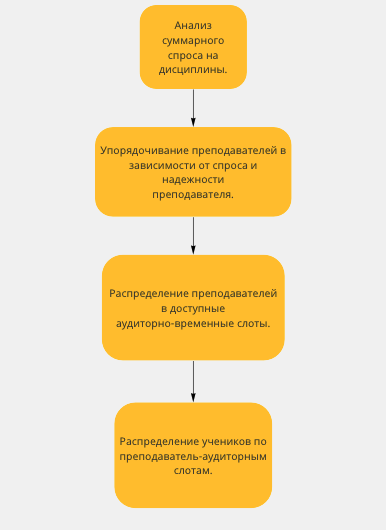
\includegraphics[width=100mm]{Images/alg_block.png}
  \caption{\textbf{Блок-схема работы алгоритма}}
  \label{alg_block}
\end{figure})\ref{alg_block}.
\begin{itemize}
    \item[Шаг 1.]  Начальная фаза: Анализ суммарного спроса на дисциплины.
    \item[Шаг 2.] Пусть даны следующие входные данные:
    
    \verb$teachersDf$: \verb$DataFrame$, содержащий информацию о преподавателях.
    
    \verb$classroomsDf$: \verb$DataFrame$, представляющий информацию о доступных аудиториях и их характеристиках.
    
Требуется распределить учителей по аудиториям, учитывая их предпочтения по времени и дисциплинам.

Для решения этой задачи используется следующий алгоритм:

Подсчитывается спрос на учителей (количество учеников) для каждого учителя и каждого класса на основе данных о студентах.
Учителя сортируются по убыванию спроса (по количеству учеников) для каждого класса.

Для каждого учителя производится поиск доступных аудиторий в соответствии с их предпочтениями по времени и дисциплинам. Если доступные аудитории не найдены в указанное время, поиск осуществляется в другое время.
Если аудитория найдена, учитель распределяется в эту аудиторию, и информация о распределении заносится в \verb$DataFrame$ \verb$distribution_df$. Аудитория удаляется из списка доступных аудиторий.

    \item[Шаг 3.] Назначение учеников в расписание: Распределение учеников по преподаватель-аудиторным слотам. 
    Для решения этой задачи используется следующий алгоритм:
    
Ученики сортируются по убыванию их "ценности" (приоритета), что позволяет приоритизировать новых учеников.
Для каждого предмета подсчитывается количество учеников в каждом классе.

Ученики сортируются в порядке убывания количества учеников в их классе и их "ценности" для каждого предмета.

Создается список доступных аудиторий для каждого ученика в соответствии с их предметом, классом и временем занятий.

Если доступная аудитория найдена, ученик распределяется в эту аудиторию, и информация о распределении добавляется в \verb$full_distribution_df$. Количество доступных мест в аудитории уменьшается на 1.

Если доступная аудитория не найдена, ученик добавляется в \verb$reserved_df$ для дальнейшего рассмотрения или перераспределения.

По завершении работы функция возвращает два \verb$DataFrame$:
 \verb$full_distribution_df$, содержащий информацию о распределении учеников, и \verb$reserved_df$, содержащий информацию о не распределенных учениках.
\end{itemize}

Алгоритм реализован на языке Python с использованием библиотеки pandas для работы с данными в формате $DataFrame$. Он выполняет распределение учеников по доступным аудиториям с учетом их предпочтений и специфики занятий. 

Характеристики:
\begin{itemize}
    \item Процессор: Apple Silicon M2
    \item Память: 8 ГБ
    \item Хранилище: 512 ГБ
\end{itemize}


\section{Результаты}



\section{Заключение главы}
В ходе работы были выполнены следующие этапы:

\begin{enumerate}
    \item Проанализирована NP-сложность задачи формирования групп обучающихся на основе проведенных исследований.
    \item Разработан алгоритм "жадного" типа для эффективного распределения учащихся и составления групп с учетом различных ограничений.
    \item Алгоритм был реализован на языке программирования Python с использованием математических моделей, описанных в предыдущих разделах.
\end{enumerate}

